\documentclass[nofilelist]{cslthse-msc}
% to show a list of used packages at the end of the document, delete the nofilelist option
%\documentclass{cslthse-msc}
\usepackage[utf8]{inputenc}
\usepackage[main=british,swedish]{babel}
\usepackage{amsmath}
%\usepackage{amsfonts}
%%\usepackage{amssymb}
\usepackage{amsthm}
%\usepackage{makeidx}
\usepackage{graphicx}
\usepackage[titletoc, header, page]{appendix}
\usepackage{transparent}
\usepackage{tikz}
\usepackage{enumitem}
\usepackage{listings}
\usepackage{svg}
\usepackage{subcaption}
\usetikzlibrary{fit,positioning,shapes.geometric}

% disable spellcheck for this section
% LTeX: SETTINGS enabled=false
\lstdefinestyle{mystyle}{
  basicstyle=\ttfamily\footnotesize,
  breakatwhitespace=false,
  breaklines=true,
  captionpos=b,
  keepspaces=true,
  numbers=left,
  numbersep=5pt,
  showspaces=false,
  showstringspaces=false,
  showtabs=false,
  tabsize=2
}
\lstset{style=mystyle}
\lstdefinelanguage{jrag}[]{java}{
  morekeywords={aspect, syn, eq, inh}
}
% LTeX: SETTINGS enabled=true

\setcounter{secnumdepth}{4} % Number subsubsections
%\setcounter{tocdepth}{4} % Include subsubsections in table of contents

% used to display the used files at the end. Select nofilelist as a package option to disable this
\listfiles % initialize

%\geometry{showframe}
%better like this?
\student{Nicholas Boyd Isacsson}{nicholas@isacsson.se}
%\students{Flavius Gruian}{Flavius.Gruian@cs.lth.se}{Camilla Lekebjer}{Camilla.Lekebjer@cs.lth.se}

\thesisnumber{LU-CS-EX: 2023-79} % Magic Number! Do not change unless Birger Swahn asks you to do so!
% default is Master. Uncomment the following for "kandidatarbete"/Bachelor's thesis
%\thesistype{Bachelor}{Kandidatarbete}

\newcommand{\CR}[1]{\textcolor{green!60!black}{[\textbf{CR}:#1]}}
%\newcommand{\CR}[1]{}

% For questions to people reviewing, remove before finalizing
\newcommand{\reviewquestion}[1]{\textcolor{red!80!black}{[\textbf{Review question}:#1]}}
%\newcommand{\reviewquestion}[1]{\textcolor{red}{\begin{itemize}\item Question: #1\end{itemize}}}
%\newcommand{\reviewquestion}[1]{}

%\title{Formatting a Master's Thesis}
\title{Type Checker Generation using Reference Attribute Grammars}
\begin{otherlanguage}{swedish}
\svensktitel{Infoga den Svenska titeln här!}
\end{otherlanguage}

%\onelinetitle
%\twolinestitle
\threelinestitle
%\fourlinestitle

%\subtitle{A {\LaTeX} class}
%\company{The Corporation AB LTD Inc}
%\supervisors{John Deer, \href{mailto:jdeer@company.com}{\texttt{jdeer@company.com}}}{Don Jeer, \href{mailto:djeer@xy.lth.se}{\texttt{djeer@xy.lth.se}}}
\supervisor{Christoph Reichenbach, \href{mailto:christoph.reichenbach@cs.lth.se}{\texttt{christoph.reichenbach@cs.lth.se}}}
%\supervisor{John Deer, \href{mailto:jdeer@company.com}{\texttt{jdeer@company.com}}}
\examiner{Niklas Fors, \href{mailto:niklas.fors@cs.lth.se}{\texttt{niklas.fors@cs.lth.se}}}

\date{\today}
%\date{January 16, 2015}

\acknowledgements{
Sincere thanks to Christoph Reichenbach,
whose enthusiasm for the subject inspired me to pursue this subject
and whose guidance in matters of both implementation and writing were key to this thesis.
Additional thanks to Niklas Fors for providing several valuable insights, greatly simplifying certain components and Alexandru Dura for providing some guidance to JastAdd internals.

I would also like to thank my partner Lo-Isabel Krantz Andrée, my family, and Moritz for their support throughout the duration of this project.

%If you want to thank people, do it here, on a separate right-hand page. Both the U.S. \textit{acknowledgments} and the British \textit{acknowledgements} spellings are acceptable.
%
%We would like to thank Lennart Andersson for his feedback on this template.
%
%We would also like thank Camilla Lekebjer for her contribution on this template, as well as Magnus Hultin for his popular science summary class and example document.
%
%Thanks also go to the following (former) students for helping with feedback and suggestions on this template: Mikael Persson, Christoffer Lundgren, Mahmoud Nasser.
}

\theabstract{
%Your abstract should capture, in English, the whole thesis with focus on the problem and solution in 150 words. It should be placed on a separate right-hand page, with an additional \textit{1cm} margin on both left and right. Avoid acronyms, footnotes, and references in the abstract if possible.
%Leave a \textit{2cm} vertical space after the abstract and provide a few keywords relevant for your report. Use five to six words, of which at most two should be from the title.

  Static type checkers are a popular method for early detection of bugs in computer programs, by ensuring the correct data types are used throughout the program.
  One approach for implementing type checkers are Reference Attribute Grammars (RAGs), a formalism for specifying the static semantics of programming languages by declaring attributes on an abstract tree-representation of the program, and is used by the JastAdd meta-compilation system.

  This report contains a study on the usability of JastAdd to programmatically generate executable type checkers from syntax-directed typing rules.
  This aims to provide integration with existing compilers implemented with JastAdd, as well as a playground for type systems usable as an educational tool.

  We find RAGs to be a flexible model for syntax-directed typing rules, and our software was able to support simple values, nodes with premises placing demands on their children, and those with rules requiring type variables.
  It proved difficult to provide compile-time verification of the typing rules, and further work is required to extend the compiler to support type environments, a necessity for most real-world type systems.
}

%\keywords{MSc, BSc, template, report, style, structure}
\keywords{type checking, type theory, code generation, reference attribute grammars}

%% Only used to display font sizes
\makeatletter
\newcommand\thefontsize[1]{{#1 \f@size pt\par}}
\makeatother
%%%%%%%%%%

\begin{document}
\renewcommand{\bibname}{References}

\makefrontmatter
\chapter{Introduction} % should give the background of your work. Important parts to cover:
% Give the context of your work, have a short introduction to the area.
While writing software, developers often make mistakes.
Catching these mistakes as early as possible can prevent these bugs from ever reaching production code.
%\CR{Possible papers to cite as evidence:
%  \url{https://dl.acm.org/doi/abs/10.1145/1985793.1985889}
%  \url{https://www.usenix.org/legacy/event/sec04/tech/full_papers/johnson/johnson_html/}
%  \url{https://ieeexplore.ieee.org/abstract/document/10190394}}
%\CR{These papers add static checkers on top of existing languages to find additional bugs; you can also
%  mention statically typed languages, but those generally don't require frequent changes to the type checker implementation, so they're less
%  compelling to motivate your work.}
Type checkers are one of the most common static checking methods, ensuring that the correct data types are used.
While some languages include type checkers in their compilers, work has also been done to add static type checkers to existing languages.
This requires writing large amounts of specialised code on a per language basis, but has shown to be effective at detecting bugs\cite{10.1145/1985793.1985889}\cite{10.5555/1251375.1251384}\cite{10190394}.
Furthermore, making changes to the typing rules of a language can require extensive rewrites in many different parts of the type checker's codebase.

% Define the problem you are solving (or trying to solve).
%\CR{Prior work has already looked into pluggable type checkers.
%  Why is translating them into JastAdd interesting?
%  (aside from theoretical questions, you can also use
%  pragmatic reasons, such as integration into our courses.)}
In this thesis we examine the feasibility of automating the writing of type checkers, based on the formal definition of the language's typing rules, using JastAdd's implementation of Reference Attribute Grammars (RAGs).
JastAdd is an interesting target because it has already been used to implement compilers of several languages, to which our typing rule implementations could be integrated.
JastAdd is also used extensively in courses at the department of computer science at LTH, where our project could serve as an educational tool, providing students an interactive way to define and test simple type systems.

Typing rules form a complex, often ambiguous, and infinite relation.
To be able to translate them into JastAdd code, we will need to define a limited subset of syntax-directed typing relations.
We identify a number of different kinds of typing rules, used in previous work in the field\ref{Pierce}, which share a common set of features for us to implement.
We then devise a strategy to translate these rules into snippets of iterative Java code, which can be evaluated by JastAdd.

%\CR{Make clear to the reader what the challenges are:
%      How are these two formalisms similar, how do they differ (at a high level)?
%      You can use a simple typing rule as an example if it helps (very optional).
%      Hint: look at determinism in evaluation (syntax-directedness), unification, but stick to intuition in this chapter; you can elaborate in Chapter 2 or later if you think it helps.}

\CR{Usually you then put a high-level summary of the rest of the thesis here (not mentioning chapters yet), something like ``we examine X and Y and introduce a strategy for Z.
  We evaluate the approach against Foo, and demonstrate Bar.
  Our case studies show Quux.
  Overall, this initial exploration shows \ldots''}


% Specify your contributions. What does this particular work/report bring to the research are or to the body of knowledge?
\section{Research questions}
To formulate our goals more concretely, we have set out to answer the following research questions:
%\CR{Give the RQs numbers so you can refer to them later.  Common form: RQ1, RQ2 etc.; some authors use RQ2.3 if they split RQ2 into multiple subquestions (this can happen later).}
\newcommand{\rqone}{RQ1: What kinds of typing rules can we translate using RAGs?}
\newcommand{\rqtwo}{RQ2: How can we implement the translations and what algorithms should we use for the output code?}
\newcommand{\rqthree}{RQ3: What are the challenges in translating typing rules into JastAdd-based RAGs?}
\begin{itemize}
  \item \rqone
    %\CR{``kinds'' of typing rules: right now the reader isn't aware that there even are different kinds (see my earlier comment on ``what the challenges are''-- sketching this out should suffice.)}
  \item \rqtwo
    %\CR{What does ``form'' mean, here?  How broad is ``implement''-- are you talking algorithms (which I think you are) or including technical challenges (which I think you have in the next RQ)?}
  \item \rqthree
    %\CR{I'd go with `challenges in translating' instead of `potential issues of translating', language-wise}
\end{itemize}

\section{Chapter outline}
%\CR{%paper $\to$ thesis; also,
 % this always comes at the very end of the introduction}
The rest of this thesis is outlined as follows.
% This chapter introduces the
Chapter 2 presents the necessary background information for the report.
Chapter 3 describes the design and implementation of our program, followed by demonstrations of its results in chapter 4.
Chapter 5 discusses the results in a more general sense, before the conclusion in chapter 6.


\chapter{Background}
%\section{Theory} % should contain the theoretical background needed to understand your work, if necessary.
\CR{General: the first paragraphs should explain what the chapter is about and how/why it is relevant, at a high level.  The reader should come out of it thinking ``I know why I want to read this''}
This chapter aims to provide all the background information required to understand the work presented in the rest of the report.
Section \ref{abstractsyntaxtrees} explains abstract syntax trees, a simplified tree-based representation of a program, suitable for performing static analysis on.
These are extensively utilised in almost every stage of our project, both in terms of our implementation and the input to the program.
%\CR{Consider saying just a little more about them here, for readers who have no idea what ASTs are and why they matter for
%    analysing programs.}
Section \ref{typetheory} details type systems,
%\CR{Too much detail in the following:}
by explaining each of the component pieces, followed by a description of their use within static type checking.
%\CR{You can use \texttt{\textbackslash label\{labelname\}} and \texttt{\textbackslash ref\{labelname\}} to reference (sub)secttions, that's usually clearer than ``next section''.}

\section{Abstract syntax trees}\label{abstractsyntaxtrees}
\CR{What's a syntax?}
An abstract syntax tree (AST) is a tree-based representation of the syntax of a program.
Each node in the tree represents a syntactic construct of the language, such as expressions, statements or declarations and the branches represent the structure.
It is abstract in that it neglects to include all the concrete details of the syntax, but rather focuses on the structure of the program.
Structural elements of the source code, such as parenthesis, commas and brackets, are no longer necessary, as the structure of the tree conveys this semantic information.

This makes it easier to write analysis based on the behaviour of a program, without concerning oneself with its exact formulation.
Several different formulations of a program with identical behaviour may be abstracted into identical ASTs.
The hierarchical structure of the tree lends itself especially well for recursive analyses, and eases the passing of information between connected structures by connecting them as parent and children nodes.
%\CR{what is ``this information'', concretely?}
A statement like \verb|if (true) then {1} else {0}| maybe instead be represented by an if-else node, with named branches pointing towards the condition and the two values.
%\CR{You could show an example, but at the very least I would like to read an argument for why the hierarchical structure of a tree is helpful.}
%\CR{You can find common examples for showing the value of ASTs over concrete syntax trees in the EDAN65 slides.}

\CR{Consider giving the syntax of a simple expression language in BNF here, since you're already discussing ``Type syntax'' later.}
\begin{figure}[h]
\begin{lstlisting}[]
Expr   -> Expr "+" Term | Term
Term   -> Term "*" Factor | Factor
Factor -> Int | "(" Expr ")"
\end{lstlisting}
  \caption{\reviewquestion{One like this? I'm unsure how to tie it in effectively.}}
  \label{typesyntaxspec}
\end{figure}

\section{Type theory}\label{typetheory}
In this section we will discuss the elements of type theory required to understand this thesis.
Firstly, we will discuss what types are and give some examples of their use.
Next, we will describe type systems, which form a relation between types and expressions.

\section{Values and expressions}
The main purpose of most computer software is to handle and manipulate data.
Each of these individual pieces of data is a value, which could be anything from the number 4 or the text `Hello!'.

Expressions are a broader term, indicating any syntactic structure which evaluates to a value.
This includes but is not limited to values, which evaluate to themselves, but also constructs of values, operators or function calls, etc.

\subsection{Data types}
%\CR{think about the connection between types and values here.  You may even want to talk about values in a separate subsection.}
Data types can be considered a categorisation of values which share common properties, such as supporting numerical operations or accessing a certain element in a list of characters.
%several different types of data in one program, such as numbers or text.
Most programming languages come with a number of built-in data types, from different kinds of numbers (integers, floating point) to strings or lists and arrays.

%\CR{if you discuss values, you can use the intuition of ``grouping values'' by certain properties (such as supported operations) to make your point clearer.}
Different parts of programs may have different constraints on the types of expressions, such as a print function requiring a string of text, or a plus function requiring some kind of number.
%\CR{Very good point about types of expressions, but again, this is likely easier to understand by linking expressions and values.
%  I strongly recommend using a definition of the form ``all values are expressions, but not all expressions are values''.}

\subsection{Type checking}
Verifying that these constraints are upheld can assist us in catching programming mistakes, preventing the wrong data types from being used in the wrong places, which may have lead to erroneous or unpredictable behaviour.
There are two main approaches to ensuring the constraints are upheld, dynamic and static type-checking.
As our project generates a static type checker, we will focus our explanations on that topic, but provide a quick overview of their differences here.
%\CR{Why would we even want to ensure that they are upheld?}

Dynamic checking is done performed runtime, with each type checked only when needed.
While this means no checks are performed unnecessarily, it makes it harder to verify the constraints over the whole program, as it won't be tested until each specific part is executed.

Static checking is performed on the code before it is run, usually as part of compilation, preventing many faulty programs from being run at all.
However, since it lacks knowledge of what happens at runtime, it's required to take a more conservative approach, flagging potential errors even in code which will never executed.
Static checkers analyse the structure of the source code, often in the form of an abstract syntax tree.

%\CR{Why would I want static checking?  Dynamic only checks when needed, isn't that more efficient?}

\CR{One mental image that helped me a lot to understand types is to see values  on one side (let's say on the left) and their types on the other (let's say the right).
  For each concrete (and possibly very complex) operator on the left-hand side (e.g., $(+)$), we then get a small number of typing rules on the right-hand side.
  This symmetry between ``concrete'' and ``abstract'' only works if you make values part of your cast of characters for this discussion.
  The value of this mental image to your approach then becomes immediate: since operators correspond to AST nodes and typing rules are abstractions over operator behaviour, typing rules will abstract over the program semantics that are captured by individual AST nodes.
}

\subsection{Type systems}
A type system typically consists of two parts, a type syntax, describing the available types of a language; and typing rules, denoting how types should be assigned to expressions within the language.
%\CR{Why do the types need a syntax?
%    (There are other approaches to types; for your own sanity, I recommend deferring to Pierce here and calling this ``typical approaches'')}

\subsubsection{Type syntax}
A type syntax, or set of types, is a definition of the valid types within a language.
\CR{Is ``type syntax'' what Pierce calls it?  Not sure I've heard that term before; I don't think it's wrong, personally, but please check in case he uses a different term.}
\reviewquestion{I believe Pierce simply refers to it as the "set of types". I seem to have got the term type syntax from EDAP15 \url{https://fileadmin.cs.lth.se/cs/Education/EDAP15/2022/web/skills/type-system.html}. In my opinion it works better to have a clear name for it, so I'm keeping it for now, unless you have further thoughts.}
It can consist of fundamental types, such as integers or booleans.
There may also be parameterised or composite types, for example lists may have a type parameter defining what values it can contain.
This enables differentiating lists that store integers from those that store strings, and ensuring that any item added to a list must be of the same type as the type parameter.
%\CR{A bit vague; consider giving an example.}
\begin{figure}[h]
\begin{lstlisting}[]
abstract Type;

Bool : Type;
Int  : Type;
\end{lstlisting}
  \caption{Type syntax consisting of two types, for boolean and integer values, written as a JastAdd AST specification (see Section \ref{astdef})}
  \label{typesyntaxspec}
\end{figure}

\subsubsection{Typing rules}
The typing relation, notated \lstinline{t : T}, is the link between the expressions of a language and the types of the type syntax.
%\CR{It is \emph{the} link, even.}
The left-hand side is an expression in the object language, typically written in its native syntax, the right-hand side a type from the aforementioned type syntax.

Typing rules are a manner of inference rules, which in their simplest form, consist of no more than a typing relation.
The typing rule \lstinline{T-True} seen in Figure \ref{typingruleexampletrue}, for example, simply assigns the type of \lstinline{Bool} to the expression \lstinline{true}.
Additionally, the typing rules in these examples have a name, given in parentheses next to the rule, though this is merely for reference.

\begin{figure}[h]
  \begin{equation}
    \tag{T-True}
    \text{true} : \text{Bool}
  \end{equation}
  \caption{Typing rule for a true value}
  \label{typingruleexampletrue}
\end{figure}

Typing rules may also have premises, a number of conditions that must hold for the typing rule to apply.
%\CR{\emph{that} must hold (``which'' relates a set to a superset: ``carrots, which are vegetables'', while ``that'' restricts a set to a subset: ``vegetables that are carrots'')}
The notational convention here is to put the premises above a bar, with the conclusion underneath it.

\begin{figure}[h]
  \begin{equation}
    \tag{T-If}
    \frac{
      t_1 : \text{Bool}\quad
      t_2 : \textsf{T}\quad
      t_3 : \textsf{T}
    }{
      \text{if } t_1 \text{ then } t_2 \text{ else } t_3 : \textsf{T}
    }
  \end{equation}
  \caption{Typing rule for an if-expression}
  \label{typingruleexampleif}
\end{figure}

\newcommand{\ty}[1]{\textcolor{blue!20!black}{\textsf{#1}}}
\newcommand{\tyvar}[1]{\textsf{#1}}
Figure \ref{typingruleexampleif} shows an example rule, typing an if-expression.
The bottom line, the conclusion, contains the keywords of the if-expression and three free variables $t_i$ which represent any term within the language.
Above the bar are three premises, placing constraints on the three variables, which must hold for the typing rule to apply.
The first constrains $t_1$ to the type bool, the second two constrain $t_2$ and $t_3$ to a type variable \tyvar{T}, which represents any single arbitrary type within the type syntax.
While \tyvar{T} may be any type, it must consistently be the same type within any single evaluation of the rule, i.e. the two terms must have the same type.
This \tyvar{T} also appears in the conclusion, as the resulting type of the if-expression, meaning the result of the entire expression will be that of the $t_2$ and $t_3$ terms.
%\CR{Consider typesetting T differently, e.g. as \tyvar{T}}
%\CR{\tyvar{T}, $t_1$, $t_2$, $t_3$ are \emph{free} variables here, logically speaking}.

\subsubsection{Evaluating typing rules}
While performing static type checking, the typing rules form the basis of our analysis.
By analysing the program, we attempt to match the syntactic form with the typing rules, to find the type of the expression.
If no matching typing rules can be found, a type error is produced.

The simplest program possible with the typing rules T-True and T-If, consists of the single value \lstinline{true}.
It can immediately be matched to the rule T-True, giving the type \lstinline{Bool}.

A slightly more complex case can be expressed as \lstinline{if true then true else true}.
The only rule that matches the structure, is T-If, with \lstinline{true} values taking the place of each of the $t_i$ variables.
To evaluate this rule, we are thus required to recursively evaluate the types each of our $t_i$ variables, to ensure they match the premises.
In this case, the type of $t_1$ evaluates to \lstinline{Bool}, matching the first premise of T-If.
The types of both $t_2$ and $t_3$, represented as the type variable \tyvar{T}, also evaluate to \lstinline{Bool}.
Since both the uses of this type variable within the premises are consistent, all three of the rule's premises have been fulfilled, and the entire expression can be typed as \tyvar{T}, which has been found to correspond to \lstinline{Bool}.

\begin{figure}[h]
  \begin{equation}
    \tag{T-Zero}
    \text{zero} : \text{Int}
  \end{equation}
  \caption{Typing rule for a zero value}
  \label{typingruleexamplezero}
\end{figure}

Adding a second value of a different type allows us to express incorrectly typed programs, for example the program \lstinline{if zero then zero else true}.
Recursively evaluating this according to T-If, we find that the premise concerning $t_1$ no longer upholds, as the type of it now evaluates to \lstinline{Int}.
Additionally, the type variable \tyvar{T} typed by both $t_2$ and $t_3$ now has contradictory use, being assigned both as the type \lstinline{Int} and \lstinline{Bool}.
As this program cannot be found to satisfy any set of typing rules in our type system, it is found to be invalid.

%\CR{Please explain the purpose of typing rules in static type checking.  Using just your two examples you would be able to show a well-typed program, and if you add one more rule (e.g. for integers), you can show a type error.  No need to build the full derivation tree, but it's important to mention recursion here.  This entire bit may be worth a separate subsubsection.}

\section{Reference Attribute Grammars}
This section introduces the subject of Reference Attribute Grammars (RAGs), first explaining the theory behind them, then introducing JastAdd, an implementation of RAGs within a Java meta-compilation system\cite{JastAdd}.

\subsection{Reference Attribute Grammars}
Reference Attribute Grammars are an extension to Attribute Grammars (AGs), a formalism used for specifying the static semantics of programming languages.
%\CR{Generally only for the static semantics (RAGs can also do dynamic semantics, if you allow circular attributes, but that's not worth mentioning here.)
%Please also connect ``semantics'' to ``type checking'' (via ``static semantics'')}
AGs provide a systematic way to define computations on the nodes of an abstract syntax tree, associating attributes with language constructs and are commonly used in the context of compiler construction, where they help define the translation of source code into executable code\cite{AGs}.

RAGs extend these properties by introducing a new kind of attribute, allowing references to other nodes in the AST, and through the references accessing the attributes of other nodes.
This provides a simplified and more flexible method for interconnectedness between nodes\cite{RAG}.

\subsection{Non-Terminal Attributes}
\cite{higherorderattributegrammars}
\CR{Your example uses Non-Terminal Attributes (NTAs) \url{https://dl.acm.org/doi/pdf/10.1145/74818.74830}, which are
not a necessary feature for RAGs.  Please introduce them in a separate section: you can very directly connect them to the idea of ``type syntax''.}

\subsection{JastAdd}
JastAdd is an implementation of RAGs for Java, offering a flexible system for writing language analysis in an object-oriented fashion.\cite{JastAdd}
Our project uses it both for the implementation of our compiler and as a compilation target, as it outputs JastAdd code.
%\CR{It's worth telling the reader here why you are explaining some details about JastAdd.}

\subsubsection{AST specification}\label{astdef}
One of the key components of a JastAdd projects are the \lstinline{.ast} files, which declare the structure of the abstract syntax tree.
This specification is then used by JastAdd to generate Java classes representing the nodes of the AST.
These AST classes can have a variety of forms, supporting both abstract classes and subclasses, and can contain components such as Java types, tokens and child nodes, and these components may also be optional or list components.
For a detailed overview of the syntax, see the reference manual\cite{jastaddref}.

\subsubsection{RAG Modules}
\begin{figure}[h]
\begin{lstlisting}[language=jrag]
aspect TypingRules {
  syn Type Zero.type() {
    return new Int();
  }
}
\end{lstlisting}
  \caption{Snippet of a .jrag file, declaring a type attribute for the Zero AST node}
  \label{boolstrgen}
\end{figure}
The RAG modules written in \lstinline{.jrag} files, declare the attributes to be included in the classes generated by the AST specification.
The files use a syntax very similar to that of Java to declare attributes of a variety of different kinds, and the body of methods corresponds directly to Java code.

\chapter{Approach/Design} % should contain a description of your solution(s), with all the theoretical background needed. On occasion this is replaced by a subset or all of the following:

%\CR{Missing: introduction to this chapter'}
We begin this chapter with a section presenting our language for writing typing rules, an adaptation of the natural semantics used to notate typing rules in the academic context.
In Section \ref{sectionarchitecture} we proceed with presenting the overall architecture of our software, including an overview graph in Figure \ref{overviewgraph}, which may be useful to bear in mind while reading the rest of the report.
Section \ref{sectionimplementation} goes into the details of our implementation, how we generate code for different parts of the typing rules.

\section{Language design}\label{sectionlanguage}
\begin{figure}[]
\begin{lstlisting}[language=java]
ruleset = rule_list

rule_list =
    rule
  | rule_list rule

rule =
    '[' upperid ']' premises_list '---+' formula
  | '[' upperid ']' formula

premises_list =
    formula
  | premises_list ',' formula

formula = term ':' tyterm

term =
    upperid '(' term_list ')'
  | upperid '(' ')'
  | upperid
  | lowerid

tyterm =
    upperid                                              // TyVal
  | lowerid                                              // TyVar

term_list =
    term
  | term_list ',' term
\end{lstlisting}
  \caption{Syntax definition for the typing rule language}
  \label{trastspec}
\end{figure}
\CR{After reading, I would now say that it's preferable to me if you keep the language definition separate
  from its implementation.  You can use Figure 3.4 as the abstract syntax, to complement the current discussion.
  This would be before the current 3.1, then.
  An advantage of this is that you can then start your ``Architecture'' discussion (in 3.2) by mentioning
  the complex dependencies, i.e., that processing a type system specification requires you to know the abstract syntax
  of the object language as well as of the types.}


\begin{figure}[h]
\centering
\begin{minipage}{.45\textwidth}
  \centering
  \begin{equation}
    \tag{T-True}
    \text{true} : \text{Bool}
  \end{equation}
  %\caption*{Pierce syntax}
  %\label{fig:sub1}
\end{minipage}%
\hspace{.1\textwidth}\begin{minipage}{.45\textwidth}
  \centering
\begin{lstlisting}[]
[T-True]
True : Bool
\end{lstlisting}
  %\caption*{ASCII representation}
  %\label{fig:sub2}
\end{minipage}
\caption{A typing rule for the value true in natural semantic syntax on the left and its equivalent ASCII representation on the right}
\label{trexampletrue}
\end{figure}
\begin{figure}[h]
\centering
\begin{minipage}{.45\textwidth}
  \centering
  \begin{equation}
    \tag{T-If}
    \frac{
      t_1 : \text{Bool}\quad
      t_2 : \text{T}\quad
      t_3 : \text{T}
    }{
      \text{if } t_1 \text{ then } t_2 \text{ else } t_3 : \text{T}
    }
  \end{equation}
  %\caption*{Pierce syntax}
  %\label{fig:sub1}
\end{minipage}%
\hspace{.1\textwidth}\begin{minipage}{.45\textwidth}
  \centering
\begin{lstlisting}[]
[T-If]
t1 : Bool,
t2 : t,
t3 : t
-----------------
If(t1, t2, t3): t
\end{lstlisting}
  %\caption*{ASCII representation}
  %\label{fig:sub2}
\end{minipage}
\caption{A typing rule describing an if-expression in natural semantic syntax and its equivalent ASCII representation}
\label{trexampleif}
\end{figure}

%- Figure of example natural deduction rules (from Pierce?) and ASCII representation
%No infix notation
%No environments

To express typing rules, we have defined an ASCII representation of the natural semantics syntax used by Pierce\cite{Pierce}.
Our language can express a subset of the notation used by Pierce, with some differences.

The largest difference lies in the notation used for the expression to be typed, where Pierce uses the object language's native syntactic form, whereas our representation is based on the corresponding AST nodes.
Node names are consistent with those used by JastAdd, followed by parentheses containing variable names to denote their child nodes in the order of their definition.
This change is necessary to allow us to type arbitrary languages without needing to understand their syntax and grammar, though it does make translating rules from one syntax to the other less straightforward.

Another difference is the use of the type variables, which have been made lowercase.
This disambiguates them from the concrete types, which as AST nodes themselves are written with uppercase letters, and also aligns the syntax for type terms with that of regular terms, where concrete nodes are written uppercase and variables in lowercase.
\lstinline{T}, which has been switched to the lowercase \lstinline{t} in order to distinguish concrete types and type variables.
This disambiguates them from the concrete types, which as AST nodes themselves are written with uppercase letters, and also aligns the syntax for type terms with that of regular terms, where concrete nodes (such as \lstinline{If}) are written uppercase and variables (\lstinline{t1}, \lstinline{t2}, \lstinline{t3}) in lowercase.
%\CR{I generally recommend avoiding the passive voice, but the use below is an example that would be OK}
Commas are also used to separate the premises, and the horizontal line separating premises from the conclusion is represented as a series of dashes.

%\CR{Optional: you can mention Alexandru's paper about how one could add metavariables into ``native'' syntax: \url{https://dl.acm.org/doi/pdf/10.1145/3485542}
%  (since this part has already been done, it's not something you needed to explore)}
%\CR{Capitalising the AST node types is consistent with their naming in JastAdd-- worth pointing out.}

%\CR{either forward reference to the discussion of the limitations, or remove the ``limitations'' bit here (you already say ``subset'', after all) and discuss those limitations after you define the language.}

Figures \ref{trexampletrue} and \ref{trexampleif} show two rules from Pierce in both their original syntax and our ASCII representation side by side.
The former figure describes a simple rule named T-True, which assigns the \lstinline{true} expression the type \lstinline{Bool}.

%\CR{Given that it's nontrivial to separate out the different changes, I recommend first enumerating the differences abstractly and then discussing how the changes manifest in the figures, rather than starting with the figures to ``derive'' the differences.}
Looking at the notation of the typed expressions in Figure \ref{trexampletrue}, the difference is minor, the syntactic term \lstinline{true} has been replaced by the name of the AST node \lstinline{True}.
The notational change is more apparent in Figure \ref{trexampleif}, where instead of the full native syntactic form, the expression is written as an AST node with its children represented as parameters.
%Note the difference between the \lstinline{true} written in Pierce, representing the native syntactic form of the expression, and the \lstinline{True} in the ASCII representation, representing the name of the corresponding AST node.
%This difference is more apparent in Figure \ref{trexampleif}, where instead of the full syntactic form, the expression is written as an AST node with its children represented as parameters.


%\CR{Important: this affects numbers used at the type level only (which is an advanced feature mostly used in undecidable
%  typesystems like the Calculus of Constructions), and it wouldn't matter here since you can't use \ty{Succ} as a parametric
%  type anyway (cf. igure 3.4).
%  My problem is that right now this reads as if you can't typecheck programs with Integer literals,
%  but those would be e.g. \textsf{Integer} AST nodes, which (to my reading) you would have no trouble writing typing rules for.
%  (you never need to touch the actual lexeme that contains the character string that encodes the integer, in traditional
%  type analysis).  So you shouldn't actually have any real-life problem here.}
%Numerical values have not been implemented, but natural numbers can be expressed using Peano numbers\cite{peano}, utilising a zero value and successor function which represents the number incremented by one.
%If a language has the syntax \lstinline{0 + 1} it may instead be represented as \lstinline{Add(Zero, Succ(Zero))}.

\section{Architecture}\label{sectionarchitecture}
In this section we will be presenting our architecture.
%Since it contains many different components, it may be helpful to refer to the overview graph in Figure \ref{overviewgraph} while reading.
Figure \ref{overviewgraph} provides an overview of all the components and the connections between them.
The rest of the section goes into further detail about individual components.

%\CR{Stylistically, technical documents should avoid discussing the process of reading (it's not as frowned upon as speaking directly to the reader, though), so I recommend just saying that the figure ``provides an overview over...''}
%\CR{Please put the following in the caption of th/e figure instead.}
%It uses rectangular boxes to represent the concrete data or artefacts of the procedure, and elliptical boxes to represent the actions performed with them.

%\CR{You still want an introduction to this section that explains what is following and why}

\begin{figure}[]
  \resizebox{\textwidth}{!}{%
  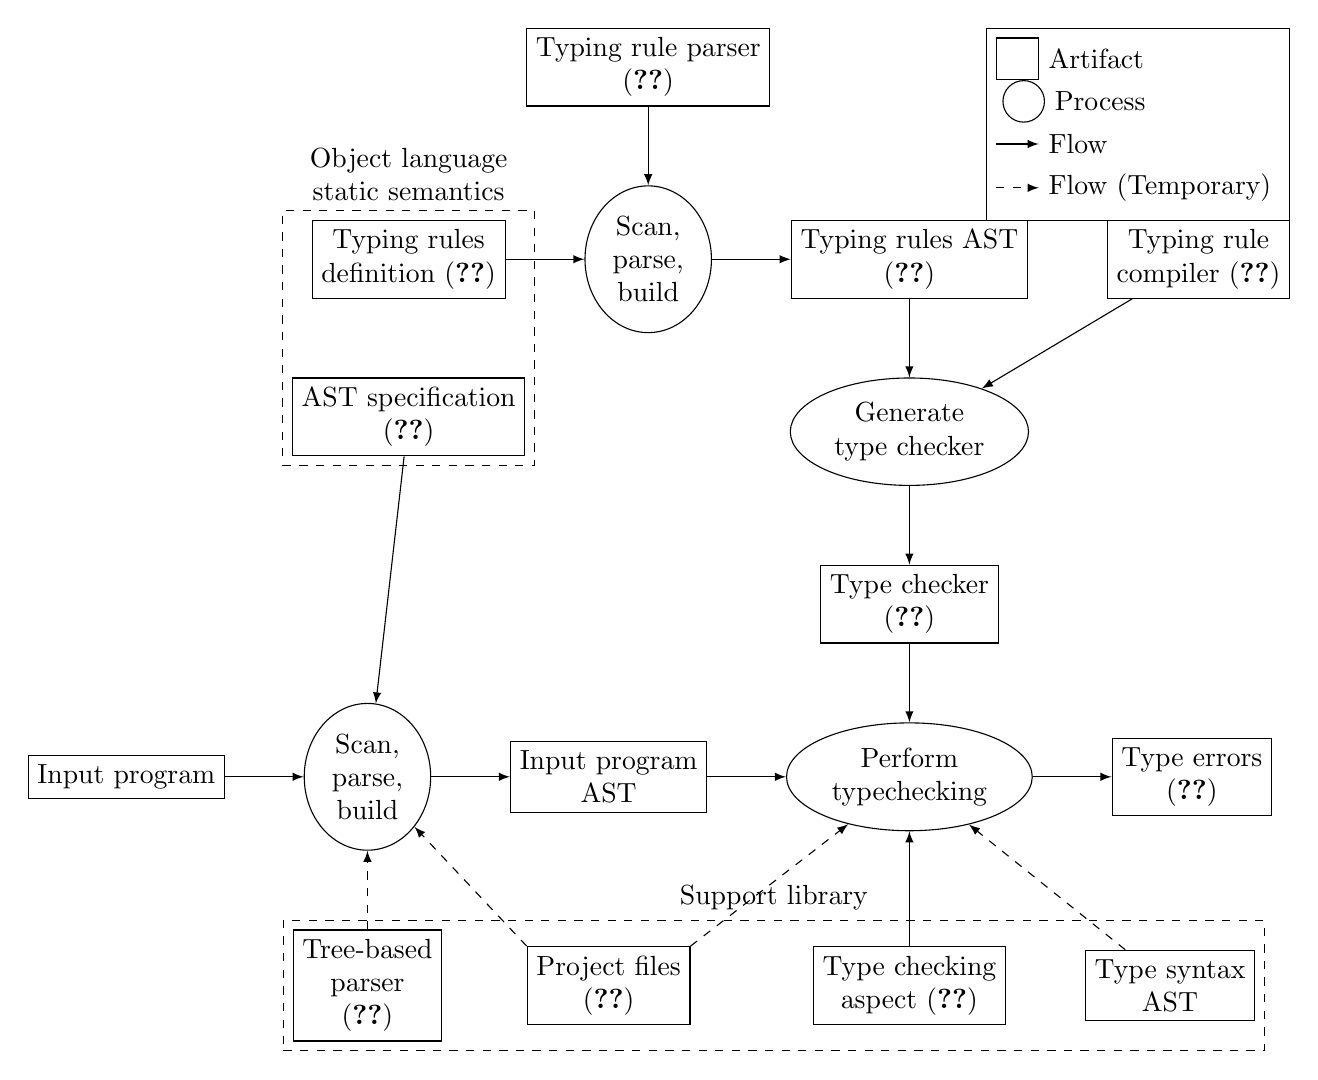
\begin{tikzpicture}[
      every node/.style = {draw=black, align=center},
      every path/.style = {draw, -latex},
      artifact/.style={draw=black},
      process/.style={ellipse}
      %greennode/.style={shape=circle, draw=green, line width=2},
      %rednode/.style={shape=circle, draw=red, line width=2}
    ]
    \node (typerules)                               {Typing rules\\definition (\ref{typingruledefinition})};
    \node (trparsing) [right=of typerules, process] {Scan,\\parse,\\build};
    \node (trparser)  [above=of trparsing]          {Typing rule parser\\(\ref{typingrulesparser})};
    \node (trast)     [right=of trparsing]          {Typing rules AST\\(\ref{typingrulesast})};

    %\node (typecheckgen) [below=of trast, process, text width=5cm] {
    %  \textbf{Type checker generation}\\
    %  \hrule
    %  \begin{itemize}[noitemsep,topsep=2pt]
    %    \item Copy template
    %    \item Generate type checker from typing rules
    %  \end{itemize}
    %};
    \node (typecheckgen)       [below=of trast, process] {Generate\\type checker};
    \node (typingrulecompiler) [right=of trast]          {Typing rule\\compiler (\ref{sectionimplementation})};
    \node (typechecker)        [below=of typecheckgen]   {Type checker \\(\ref{typecheckingalgorithm})};

    \node (olast)     [below=of typerules] {AST specification\\(\ref{astdef})};

    \node (outputtypechecking) [below=of typechecker, process] {Perform\\typechecking};
    \node (inputast)           [left=of outputtypechecking]    {Input program\\AST};
    \node (outputparsing)      [left=of inputast, process]     {Scan,\\parse,\\build};
    \node (typeerrors)         [right=of outputtypechecking]   {Type errors\\(\ref{errorhandling})};
    \node (inputprog)          [left=of outputparsing]         {Input program};

    %\node (template) [below=of inputast, text width=6cm] {
    %  \textbf{Type checker template}\\
    %  \hrule
    %  \begin{itemize}[noitemsep,topsep=2pt]
    %    \item Scanner, parser, builder
    %    \item Project files
    %    \item Type checking algorithm (\ref{typecheckingalgorithm})
    %  \end{itemize}
    %};
    \node (templateparser)        [below=of outputparsing]                               {Tree-based\\parser\\(\ref{treebasedparser})};
    \node (templateprojectfiles)  at (inputast |- templateparser)                        {Project files\\(\ref{projectfiles})};
    \node (typecheckingalgorithm) at (outputtypechecking |- templateparser)              {Type checking\\aspect (\ref{typecheckingaspect})};
    \node (templatetypesyntax)    [right=of typecheckingalgorithm]                       {Type syntax\\AST};
    \node (template)              [dashed, fit=(templateparser) (typecheckingalgorithm) (templatetypesyntax)] {};
    \node                         [above, draw=none] at (template.north)                 {Support library};

    \node (userinput)   [dashed, fill=none, fit=(typerules) (olast)]                  {};
    \node               [above, draw=none] at (userinput.north)                       {Object language\\static semantics};
    %\node (typechecker) [dashed, fill=none, fit=(outputparsing) (outputtypechecking)] {};
    %\node               [above, draw=none] at (typechecker.north)                     {Type checker};

    \draw (typerules)          to (trparsing);
    \draw (trparser)           to (trparsing);
    \draw (trparsing)          to (trast);
    \draw (trast)              to (typecheckgen);
    \draw (typingrulecompiler) to (typecheckgen);
    \draw (typechecker)        to (outputtypechecking);
    \draw (olast)              to (outputparsing);
    \draw (outputparsing)      to (inputast);
    \draw (inputast)           to (outputtypechecking);
    \draw (outputtypechecking) to (typeerrors);
    \draw (typecheckgen)       to (typechecker);
    \draw (inputprog)          to (outputparsing);

    \draw[dashed] (templateparser)                  to (outputparsing);
    \draw         (typecheckingalgorithm)           to (outputtypechecking);
    \draw[dashed] (templateprojectfiles.north west) to (outputparsing);
    \draw[dashed] (templateprojectfiles.north east) to (outputtypechecking);
    \draw[dashed] (templatetypesyntax)              to (outputtypechecking);

    \matrix [below left, nodes={minimum size = 15pt, align=left}, align=left] at (current bounding box.north east) {
      \node [artifact, label=right:Artifact] {}; \\
      \node [process, label=right:Process] {}; \\
      \node [draw=none, label=right:Flow] (leg1){}; \\
      \node [draw=none, label=right:Flow (Temporary)] (leg2){}; \\
    };
    \draw [label=right:Line] (leg1.west) to (leg1.east);\\
    \draw [dashed, label=right:Dashed] (leg2.west) to (leg2.east);\\

  \end{tikzpicture}
  }
  \caption{An overview of the project components and flow.
It represents the flow of the program, with components and artefacts (represented as rectangular boxes) with arrows linking them to actions (elliptical boxes) which in turn have arrows to the new components and artefacts they produce.
The dashed arrows from represent links from the support library components that exist in the current experimental state of the project, but in a finished product would instead link to component from the object language's own compilation environment.
  \CR{Can you mark, e.g. via colours, the parts that the user provides,
           and the parts that will be in the generated output project?}}
  \label{overviewgraph}
\end{figure}

\subsection{Typing rule definition}\label{typingruledefinition}
To express typing rules, we created a simple ASCII representation of the natural deduction notation used by Pierce\cite{Pierce}.
Custom DSL
Include typing rules AST specification (or BNF?)
ASCII representation of natural deduction %BNF (is it BNF?)


\subsubsection{Typing rules parser}\label{typingrulesparser}
The parser for typing rules is written using JFlex\cite{jflex}, a scanner generator, and Beaver\cite{beaver}, an LALR parser generator.
JFlex takes a series of regular expressions to generate a tokenizer for the parsed language.
The tokens are passed on to Beaver along with a parser definition in extended Backus-Naur form (EBNF), to generate a parser.


\subsubsection{Typing rules AST}\label{typingrulesast}
%\CR{I would give this AST/BNF a more specific name here, to distinguish it from the other two (as done nicely already in Figure 3.1)}
\begin{figure}[h]
\begin{lstlisting}[]
RuleSet ::= Rule*;

Rule ::= <Name> Conclusion:Formula Premises:Formula*;

abstract Formula;
HasType : Formula ::= Expr:Term Ty:TyTerm;

abstract Term;
Function : Term ::= <ID> Term*;
Value    : Term ::= <ID>;

abstract TyTerm;
TyVal : TyTerm ::= <ID>;
TyVar : TyTerm ::= <ID>;
\end{lstlisting}
  \caption{Typing rules abstract syntax tree specification}
  \label{trastspec}
\end{figure}
%\CR{The syntax doesn't allow parametric types; please make that explicit here.}

The abstract syntax tree for the typing rules language consists of a \lstinline{RuleSet} root node.
The root node contains only a list of rules, where each rule has a name, a conclusion and a list of premises.
The rule's name is currently unused but is intended to be utilised in error reporting, to clearly specify what rules are available for each node, or which rule is causing an error.

Both conclusion and premises are represented by the abstract HasType node, consisting of a term, which may be a function or value; and a typeterm, representing either a type value or a type variable.
For the conclusion, this node represents what type should be assigned to the term on the left, whereas for the premises, the node represents a requirement for the node on the left to have the type on the right.

Currently, our compiler does not support type parameters, so they are not included in the AST.
To support this in future, an additional \lstinline{TyTerm} could be added which includes a list of \lstinline{TyTerm}s along with its ID.

\subsection{Support library}
In addition to the generated type-checking files, there are a number of files that are added to the output file that are identical for all generated type checkers, which we refer to as the support library.
Some of these are key components of the type checker, but others are dummy components included solely for convenience of testing.
We expect that in a real world use case, our software would integrate into an object language's compiler pipeline, and utilise its own parser and project files to provide the abstract syntax tree for our type checking to tie into.
For testing purposes, we have written generic versions of these components, which work for any supported object language.
%\CR{``Templates'' are usually things that are mostly fixed but have holes to be filled in.  I would call what you describe here the ``support library''}

\subsubsection{Input program parser}\label{treebasedparser}
%\CR{Parser for what?}
%\CR{Is there a conection between this section and Section~\ref{typingrulesparser} wrt parsing terms of the object language?}
For testing purposes, our support library comes with a generic tree-based parser.
Programs are written as a tree of AST node names followed by potential parenthesis within which a comma separated list of child nodes are written.
The parser parses the tree recursively, using Java's reflection API to find a class with a matching name, and a constructor with parameters of the same amount and types.
Figure \ref{boolinputexample} shows an example input file for the Bools language, which will be discussed further in Section \ref{boolsast}.

\begin{figure}[h]
\begin{lstlisting}[]
Expression(
  Or(
    True,
    Or(
      True,
      False
    )
  )
)
\end{lstlisting}
  \caption{Example tree-representation input for the Bools language}
  \label{boolinputexample}
\end{figure}

This approach does have the issue of occasionally parsing invalid programs, due to the reflection API finding an additional parameterless default constructor.
This leads the parser to always accept nodes written with no children, such as \lstinline{Expression(Or())}, even if the AST specification requires them.
These children will be null, causing issues further down the line, though as this parser is only intended for testing it is of little concern.
%\CR{Does this also apply to the analysis of typing rules?  If so, you can mention it as ``future work''
%  or describe how it could be fixed (it's not a fundamental limitation, so nothing that warrants a deeper discussion)}

\subsubsection{Project files}\label{projectfiles}
For ease of use the compiler will output a complete runnable Gradle project.
It can parse simplified tree-representations of programs, and utilise these to perform the type checking.
In a future real world use case, it is intended for our generated type-checking aspects to integrate into a pre-existing project, which already has all the necessary project files to parse an AST tree, to which our type aspects could integrate.

%\CR{Can you elaborate on if/how this would integrate with an existing language implementation?
%  I've always interpreted everything as that you start with some `objectlanguage.jar' file of an existing language (given that you use reflection), and you get out a fresh Gradle project that uses that `objectlanguage.jar' for parsing and AST construction, but since you generate JastAdd source code, you can't really (to my understanding) add the `type()' attribute etc. to the existing implementation, since JastAdd needs to run over the source jrag files.
%  Going by your overview figure, I now wonder if the generated file also incorporates all of the source code of the original project?  Or do you reconstruct the AST specification via reflection somehow and simply mirror it in the generated project (which would lead to two different AST representations, but with a straightforward mapping)?}


%\subsubsection{Executable}

%\subsection{Typing rule compiler}\label{sectionimplementation}

%\subsection{Output type checker}
%\subsubsection{Tree-representation}
%\subsubsection{Type checking algorithm}\label{typecheckingalgorithm}
%Generate code for each node and typing rule
%Simple algorithm
%Recursive


%\section{Method (remove this?)} % describe how you go about solving the problem you defined. Also how do you show/prove that your solution actually works, and how well does it work.



\section{Implementation}\label{sectionimplementation} % if your work involved building an artefact/implementation, give the details here. Note, that this should not, as a rule, be a chronological description of your efforts, but a view of the result. There is a place for insights and lamentation later on in the report, in the Discussion section.

%\subsection{Type checker generation}
The type checker generation is based on a single-responsibility principle, where each node of the abstract syntax tree (of \emph{which} of the three (or four?) ASTs?) is responsible for generating the code it corresponds to \CR{Not sure what you mean}.
Once typing rules have been parsed, we end up with an abstract syntax tree, in the form of Figure \ref{trastspec}, where the \lstinline{RuleSet} is the root node.
From the root node, calls propagate down the tree to fill in increasingly specific sections of the code.

This section details the implementation of our type checker generator, on a feature by feature basis.


%\subsubsection{Aspect generation}
\subsection{Aspect generation}
The \lstinline{RuleSet} node is responsible for generating the overall structure of the output file, a JastAdd aspect called \lstinline{TypingRules}.
It sorts its \lstinline{Rule} children by which nodes they apply to, so that if multiple tying rules type the same node, they can be inserted into the same method implementation.

%\subsubsection{Method implementation overview}
\subsection{Method implementation overview}
The implementation of a typing rule can range from a single return statement to a system of declarations of variables, type variables and control flow.
These are explained in further detail in subsequent sections, but here follows a quick overview.

Firstly, the algorithm checks if the number of premises is zero, in which case it immediately generates the conclusion, consisting of a return statement.
If there are premises, it first generates code for the declarations of variables and type variables.
This is followed by an if-statement to test whether the premises hold true, containing a return statement.
Should the premises not hold, a type error is produced.
\CR{What if there are multiple rules that apply to the same AST node?  E.g., one rule that allows \ty{Int} addition and one that allows \ty{String} addition.}

%\subsubsection{Parameters}
\subsection{Parameters}
When the typing rules concern a node with parameters, these can be named arbitrarily \CR{Who does the naming?  Why is the ``arbitrarily'' bit important?}\CR{ Will this work if the type system specification has a type variable called ``this'' or ``null'' or ``class''?}, and a variable with the same name will be instantiated at the beginning of the method, fetching the corresponding child node by index.
These variables are then utilised in later premises or type variable declarations.

%\subsubsection{Premises/control flow}
\subsection{Premises/control flow}
The rule's premises are translated into an if-statement, which checks all types using a method \lstinline{matches} added to all Type nodes.

The current implementation of \lstinline{Type.matches(Type t)} checks that the Type it is called on is either of the same class or a subtype of the type \lstinline{t}.
\CR{is ``matches'' a good name for something that is not symmetric?}
This allows the language limited sub-typing at the type checker generation step, though the pros and cons of this have not been evaluated.
\CR{Can you give an example of a case where this is helpful, and one example where it might be troublesome?
Let's use the ``if'' rule as an example.  If $\ty{Number} :> \ty{Int}$ (\ty{Number} is a supertype of \ty{Int}), what type will I infer if $t_2 = \ty{Number}$ and $t_3 = \ty{Int}$?  How about the other way around?}
It is also possible to override the \lstinline{matches} implementation for a specific Type, by adding a definition to a JastAdd aspect included in the output type checker.
\CR{This sounds like this is a way to support ``ad-hoc type polymorphism''?}

%\subsubsection{Type variables}
\subsection{Type variables}
In the case of type variables, the generated code takes a dynamic approach \CR{Meaning?} to simplify the implementation.
Each type variable that appears in the conclusion is instantiated to a null value, and the code generated by each premise first checks if the value is still null and either assigns the variable its own type or tests to make sure the existing type matches its own.
\CR{Is there a hidden order dependency? (Cf. my earlier question about ``matches'')}

\CR{Overall, I am not convinced that this strategy for presenting the type checking algorithm is very effective (though it might be better for someone who is reading the source code at the same time).
  I would propose to merge 3.2.2, 3.2.3, 3.2.4, 3.2.5, and to split them into (a) the type checking algorithm (while ignoring the code generation bit), and (b) the code generation aspect.
  I.e., for (a), pretend that you are interpreting the typing rules instead of compiling them, and please try to present an algorithm that captures
  the check.
  The algorithm can be in plain English with bullet points / numbered sub-steps, or in some pseudo-formal notation (``foreach premise $p$ in rule $r$ ...''), as long as it is clear.}

\subsection{Type-checking algorithm}\label{typecheckingalgorithm}

For each rule:
\begin{enumerate}
  \item For each parameter in the conclusion:
    \begin{enumerate}
      \item Declare a variable by the same name, initialised by fetching the child of the same index.
    \end{enumerate}
  \item For each type variable used in the rule:
    \begin{enumerate}
      \item Initialise it to null
      \item Iterate through each premise it appears on the right-hand side of:
        \begin{enumerate}
          \item If the type variable is set to null, evaluate the type of the left-hand side and assign it to the type variable.
          \item If the type variable is not set to null, evaluate the type of our left-hand side and check if it is the same type or a subtype to the type variable. If it is not, throw a type error.
        \end{enumerate}
    \end{enumerate}
  \item Check whether each of the premises is true:
    \begin{enumerate}
      \item Evaluate the type of the left-hand side of the premise and check if it is the same type or a subtype to the right-hand side.
    \end{enumerate}
    If all true: Return the right-hand side of the premise
  \item Throw a type error if we reach this point
\end{enumerate}

\begin{figure}[h]
%foreach parameter in rule.conclusion.parameters:
%  declare var "parameer.name" = getChild(parameter.index)
\begin{lstlisting}[]
foreach typevar in rule.typevars
  declare typevar = null
  foreach premise in rule.premises where premise.rhs == typevar:
    if typevar == null:
      typevar = premise.lhs.type()
    else:
      if typevar != premise.lhs.type():
        throw typeerror("Type variable mismatch")

if(premise1.lhs.type() == premise1.rhs &&
   premise2.lhs.type() == premise2.rhs &&
   ...
  ):
    return conclusion.rhs
throw typeerror("Typechecking failed")
\end{lstlisting}
  \caption{Pseudocode for the implementation of the type() attribute}
  \label{boolsast}
\end{figure}
\subsection{Code generation}

\subsection{Type checking aspect}\label{typecheckingaspect}
The type checking aspect contains the declaration of the \lstinline{type()} attribute for all AST nodes, as well as a default implementation.
This default implementation immediately produces a type error, to cause an error when the type of an expression not defined in the typing rules is demanded.

%\CR{The details of this section (esp.\@ the bit below) might fit better into Section~\ref{sectionimplementation}?}
%\CR{What is ``type matching''?  I am not familiar with this term, and you haven't introduced it before.}
It also contains the implementation of the type matching method, which checks whether a type is equal to or a subtype of another type, which can be seen in Figure \ref{typematches}.
It is defined for all \lstinline{Type} nodes, and checks whether the type's class is equal to or a subclass of the parameter type.
\CR{So this is not an equivalence relation, but a partial order?  What does that mean wrt how it is used by the implementation of the type checker?} \reviewquestion{I think it would be easier to change this poorly thought out line of code than to fully evaluate and address the implications in the report :) Is that okay?}

\begin{figure}[h]
\begin{lstlisting}[language=jrag]
syn boolean Type.matches(Type t) {
  return t.getClass().isAssignableFrom(getClass());
}
\end{lstlisting}
  \caption{Definition of the type matching method}
  \label{typematches}
\end{figure}



%\subsubsection{Error handling}\label{errorhandling}
\subsection{Error handling}\label{errorhandling}
The current error handling consists of throwing a runtime exception at the first discovered type error, ceasing the type checking immediately.
This method was chosen solely for its simplicity of implementation, rather than its functionality.
Possible improvements to it are discussed in Section \ref{improvederrorhandling}.

It provides a stack trace with information on see where in the type checking code the error occurs (such as what typing rule fails), but doesn't currently provide any information about what section of the input program causes the error.
%This tends to result in errors that are more useful for debugging the typing rule implementation, rather than providing useful information to the user of the type checker, where there is much room for improvements.

%\CR{This section is needlessly apologetic-- error handling was not the focus of your work.  You can add a forward reference to 6.1.2, though.}

%Once typing rules have been parsed, we end up with an abstract syntax tree, in the form of Figure \ref{trastspec}, where the \lstinline{RuleSet} is the root node.
%The \lstinline{RuleSet} node consists of a list of \lstinline{Rule} nodes, and begins by sorting each rule by which object language node it describes.
%
%The \lstinline{RuleSet} node then begins by generating the outline of a JastAdd aspect \lstinline{TypingRules}, and the definition for the method \lstinline{.type()} for each object language node.
%It then calls on the \lstinline{Rule} node to fill in the implementation of the method.
%
%A \lstinline{Rule} consists of a name, a conclusion, and a possibly empty list of premises that need to be true for the conclusion to be returned.
%In the simplest case of an empty list of premises, the entire content of the rule is generated by the conclusion.
%For rules containing premises, the code becomes more involved.
%Firstly, any variables or type variables used in the rule need to be declared, followed by a check to ensure each use of a type variable represents a node with the same type.
%Then it generates an if-statement corresponding to our premises, by letting each \lstinline{Premise} generate a boolean expression, all of which get joined by the AND operator.
%
%Both \lstinline{Premise}s and \lstinline{Conclusion}s are represented by the same abstract class \lstinline{Formula}, which currently contains a single implementation \lstinline{HasType}, consisting of an expression and a type.
%Depending on whether it is used as a premise or conclusion, it can either represent that the expression must have the specified type or that the expression should be given the specified type.

%\subsection{Type checker design}
%The provided typing rules compile into \lstinline{type()} methods, which return a value from the Type interface.
%For the most simple typing rules, this method's implementation will consist of a single return statement.
%
%Types are declared in an AST specification, currently provided by the template, allowing simple type hierarchies.


\chapter{Evaluation} % is the part where you present the finds. Depending on the area this part contains a subset or all of the following:
In the first section of this chapter, we present typing rule definitions for a few simple type systems, alongside the resulting code produced as an output when they are input to our compiler.

In Section \ref{sectionresearchquestions}, we evaluate the overall result of our study by answering our research questions.
%\CR{The section has two parts, so the intro paragraph here can directly discuss their purpose.}
%\section{Experimental Setup} % should describe the details of the method used to evaluate your solution(s)/approach. Sometimes this is already addressed in the \textbf{Method}, sometimes this part replaces \textbf{Method}.
\section{Results} % contains the data (as tables, graphs) obtained via experiments  (benchmarking, polls, interviews). Here you should also describe the individual tables or graphs in text, pointing out interesting outliers and trends.
\CR{You can't discuss results without describing your experiments, but to describe the experiments, you should first motivate them.
  Since you are doing case studies, you can use Pierce to motivate your choice of languages (even if your language is subtly different somehow; I don't have the book in front of me).
  Make clear to the reader that you picked your languages based on the existing literature, not on a whim.}
%\subsection{Input/output examples, with descriptions}
\subsection{Bools}

\begin{figure}[]
\begin{lstlisting}[]
Expression ::= Term;

abstract Term;
True  : Term;
False : Term;
Or    : Term ::= Left:Term Right:Term;
Zero  : Term;
\end{lstlisting}
  \caption{AST specification for the Bools language}
  \label{boolsast}
\end{figure}
\begin{figure}[]
\begin{lstlisting}[]
[T-True]
True : Bool

[T-False]
False : Bool

[T-Or]
left : Bool,
right : Bool
----------------------
Or(left, right) : Bool

[T-Zero]
Zero : Int
\end{lstlisting}
  \caption{Typing rules for the Bools language}
  \label{boolstr}
\end{figure}

\begin{figure}[]
\begin{lstlisting}[language=jrag]
aspect TypingRules {

  syn Type Zero.type() {
    return new Int();
  }

  syn Type Or.type() {
    ASTNode left = getChild(0);
    ASTNode right = getChild(1);

    if(left.type().matches(new Bool()) &&
       right.type().matches(new Bool())) {
      return new Bool();
    }
    throw new RuntimeException("Typechecking failed");
  }

  syn Type True.type() {
    return new Bool();
  }

  syn Type False.type() {
    return new Bool();
  }
}
\end{lstlisting}
\caption{Generated typing rules for the Bools language (reformatted for readability)}
  \label{boolstrgen}
\end{figure}
A simple example of a language is provided in Figure \ref{boolsast}, consisting of three values, \lstinline{True}, \lstinline{False} and \lstinline{Zero}; and the boolean operator \lstinline{Or} with two parameters, Left and Right.
In the AST specification, there are no limitations on what terms can be provided as parameters to the \lstinline{Or} operator, allowing illogical constructs such as \lstinline{Or(True, Zero)}.

To prevent cases like these, we define typing rules via the specification in Figure \ref{boolstr}.
The typing rules for \lstinline{True}, \lstinline{False} and \lstinline{Zero} contain no premises and define the type as \lstinline{Bool} and \lstinline{Int} as appropriate.
The typing rule for the \lstinline{Or} operator, which takes two parameters \lstinline{left} and \lstinline{right}, contains two premises, specifying that the \lstinline{Or} operator has the type \lstinline{Bool} only if both the \lstinline{left} and \lstinline{right} terms also have the type \lstinline{Bool}.

The typing rules from Figure \ref{boolstr} generate the type definitions in Figure \ref{boolstrgen}.
The simple rule definitions for the values compile into equally simple implementations, consisting of a single return statement of a newly constructed \lstinline{Type} object.
For the \lstinline{Or} node, the code becomes slightly more complex.
\CR{The next bit would probably be easier if you just show the code.}
First two variables are defined, corresponding to the parameters in the typing rule, and assigned to the children with the index corresponding to the position among the parameters.
This is followed by an if-statement, recursively evaluating the children's types and comparing the result the type demanded in the premise.
If the condition is true, a \lstinline{Bool} type is returned.
If not, a runtime exception is thrown to convey a type error.

\CR{You may want to add a short statement that this captures the intended behaviour of the type checker.}

\subsection{If-else extension}

\CR{Separate case study or next step in the same case study?  Either way, the section title should make the connection to 4.1.1 (or lack thereof) clear.}

\begin{figure}[]
\begin{lstlisting}[]
IfElse : Term ::= Cond:Term Then:Term Else:Term;
\end{lstlisting}
  \caption{Extension for the Bools AST in Figure \ref{boolsast} \CR{Consider giving this language a different name, for clarity}}
  \label{ifelseast}
\end{figure}

\begin{figure}[]
\begin{lstlisting}[]
[T-IfElse]
x: Bool,
y: a,
z: a
------------------
IfElse(x, y, z): a
\end{lstlisting}
  \caption{Extension for the Bools typing rules in Figure \ref{boolstr} with an if-else term}
  \label{ifelsetr}
\end{figure}
\begin{figure}[]
\begin{lstlisting}[language=jrag]
syn Type IfElse.type() {
  ASTNode x = getChild(0);
  ASTNode y = getChild(1);
  ASTNode z = getChild(2);

  Type tyvar_a = null;
  if(tyvar_a == null)
    tyvar_a = y.type();
  else if (!tyvar_a.matches(y.type()))
    throw new RuntimeException("Typechecking failed: Type variable mismatch");
  if(tyvar_a == null)
    tyvar_a = z.type();
  else if (!tyvar_a.matches(z.type()))
    throw new RuntimeException("Typechecking failed: Type variable mismatch");
  if(x.type().matches(new Bool()) &&
     y.type().matches(tyvar_a) &&
     z.type().matches(tyvar_a)) {
    return tyvar_a;
  }
  throw new RuntimeException("Typechecking failed");
}
\end{lstlisting}
\caption{Generated typing rules for the if-else term, extending Figure \ref{boolstrgen} (reformatted for readability)
  \CR{The components of this function would be great to discuss in Section 3.  Here in Section 4, you may want to forward reference the discussion about redundancy/possible optimisations (Section 4.2.2) and very concretely use this code and explain the changes you have in mind (for someone else to do in future work).}
}
  \label{ifelsetrgen}
\end{figure}

%\begin{figure}
%\centering
%  \begin{minipage}[b]{.4\textwidth}
%  \centering
%\begin{lstlisting}[]
%[T-IfElse]
%x: Bool,
%y: a,
%z: a
%---------
%IfElse(x, y, z): a
%\end{lstlisting}
%  \captionof{figure}{A figure}
%  \label{fig:test1}
%\end{minipage}%
%\begin{minipage}[b]{.6\textwidth}
%  \centering
%\begin{lstlisting}[]
%syn Type IfElse.type() {
%ASTNode x = getChild(0);
%ASTNode y = getChild(1);
%ASTNode z = getChild(2);
%
%Type tyvar_a = null;
%if(tyvar_a == null) tyvar_a = y.type();
%else if (!tyvar_a.matches(y.type()))
%throw new RuntimeException("Typechecking failed: Type variable mismatch");
%if(tyvar_a == null) tyvar_a = z.type();
%else if (!tyvar_a.matches(z.type()))
%throw new RuntimeException("Typechecking failed: Type variable mismatch");
%if(x.type().matches(new Bool()) && y.type().matches(tyvar_a) && z.type().matches(tyvar_a)) {
%return tyvar_a;
%}
%throw new RuntimeException("Typechecking failed");
%}
%\end{lstlisting}
%  \captionof{figure}{Another figure}
%  \label{fig:test2}
%\end{minipage}
%\end{figure}
As an example of rules utilising type variables, we can extend the Bools language with an if-else term.
\CR{``Can extend'' sounds a bit arbitrary.  Can you motivate with Pierce (even if not exactly)?}
As shown in the AST extension in Figure \ref{ifelseast}, it consists of three terms: a conditional, a term to be evaluated if the condition is true and a condition to evaluate if false.
A typing rule of this if-else term can be seen in Figure \ref{ifelsetr}.
The rule has three premises, the first of which declares the conditional must have the type \lstinline{Bool}.
The next two declare that the two other children must be of the type \lstinline{a}, with the lowercase \CR{grammar} indicating a type variable.
This type variable \lstinline{a} also subsequently appears in the resulting type of the if-else term.

%\CR{``Shown in Figure~\ref{reference}'' is the current preferred form in our field}
The code for this rule is shown in Figure \ref{ifelsetrgen}, and begins with three parameter declarations as in previous rules, followed by a new type variable declaration on line 6, which is instantiated to null.
For each invocation of the type variable, a code section is generated, which checks if the type variable is still null, and if so assigns it to the type of the left-hand side term, or if it has been assigned checks whether the types match each other. Should any non-matches be found, a type error is thrown.

The rest of the method is similar, with premises being checked -- including a redundant check of the type variables -- before returning the type variable, or a type error being thrown.

\section{Research questions}\label{sectionresearchquestions}

\subsection*{\rqone}
Our project has shown that generating type checkers using RAGs is a viable solution for a number of different language constructs.
%To assess our implementation, we'll go through the examples used by Pierce\cite{Pierce} to see which cases we can successfully express.
To evaluate the completeness of our implementation, we refer to Pierce\cite{Pierce} as a reference work.
The typing rules are introduced in chapter 8, starting with the simple examples shown in Section \ref{sectionlanguage}.
\CR{Please be clearer on which examples from Pierce you implemented and where support stops.}
We have implemented support for simple type declarations, where a value or function always has a certain type.
These simple rules are not of much interest in themselves but are an important backbone to the subsequent analysis.
We also support type declarations with premises that must hold for the rule to apply, allowing us to express relationships between types and bringing with them the possibility of type errors.

Type variables extend these relationships further by providing a layer of abstraction, allowing us to write rules where the types are not precisely defined.
This enables rules where the return type of an expression depends on its child expressions, or where child expressions must have the same types.

A major feature missing from our implementation is the concept of type environments or typing contexts, providing a mapping from variables and functions to types.
This prevents us from generating type checkers for even simple general purpose languages.

\CR{Please explain typing contexts and why/where they are important.  You can also reflect on whether typing contexts are necessary in the context of RAG-based analysis (cf. what we did in EDAP15).}

\CR{I am missing the phrase ``syntax-directed'' here.}

\subsection*{\rqtwo}
We have approached translating typing rules into a JastAdd attribute \lstinline{type()},
%\CR{parsing is the syntactic analysis of the input specification, you have done more than just parsing.}
which either returns a \lstinline{Type} value, or throws a runtime exception if the expression is invalidly typed.

We have chosen to represent the right-hand side of type equations, the types themselves, as an abstract AST class.
While our current implementation only supports simple types, this representation gives us a lot of flexibility for future extensions.
Parametric types, such as lists where the type of the list contains information about the types of its elements, could be expressed as simply as \lstinline{MyList : Type ::= Type;}.
The current implementation of \lstinline[language=java]{matches()} would however consider all lists to match, without comparing the child nodes.
Perhaps the default implementation could be extended to compare all child elements, or these more advanced types would require manually overriding the method.
\CR{Recursive term equivalence can become tricky when you are dealing with type variables (cf. the Hindley-Milner inference exercise in EDAP15).}
\CR{Type equality could also be expressed in terms of typing rules.  This approach is quite common with subtyping.}

We have implemented premises as conditions of a single if-statement, where we check that each premise holds true before returning the type, or falling through to a type error if the premises do not hold.
It might instead be worthwhile to check each condition individually, to be able to specify in the error message precisely which premises have failed and why.
%This would perhaps make it easier to implement informative type errors, as you could report precisely which premise is failing.
If paired with the current error handling of throwing an exception to convey type errors, it would make it harder to implement having multiple valid rules providing the type of an expression, as the first failure would throw an exception, stopping the evaluation of any further typing rules which may have been successful.
%\CR{What do you mean by ``seize''?}
An alternative error handling would suit it better, one able to collect multiple errors without seizing evaluation, perhaps merely adding all the errors to a list and checking whether it is empty before returning a type.

The variables in the typing rules are compiled into regular Java variables containing the AST node.
Notably, the declarations of these variables type them merely as \lstinline{ASTNode}.
As we currently only utilise the \lstinline{type()} attribute, which is declared for all nodes, this lost information has little impact.
However, in the future it may become relevant to type these more specifically, to support more complex rules that require deeper analysis within the tree.

Type variables similarly are implemented as Java variables, though they are initiated as null, to represent the type variable's unassigned state.
This is followed by a check for each point of use in the typing rule, to see whether the type variable is still unassigned and if so assign it.
This approach could be improved by finding the first use of each type variable during the rule compilation, and generating a single declaration statement initialising it to the type of the corresponding expression.
%\CR{no need to say ``much room for improvement'', just mention the specific disadvantages.}
\CR{I am missing a discussion of type variables and unification as we used them in EDAP15 for Hindley/Milner.}

A cleaner solution to this might be view rules as a kind of pattern matching, where each rule is evaluated one by one until a matching one is found.
Instead of reporting the reason any individual rule failed, the error might instead display either all or only the best matching of the rules it tried to apply, perhaps with a list of non-holding premises for each one.
%\CR{This is a good idea; you can even sort the rules by closest matches and only show the top ones if there are many.}

\CR{Can you structure this subsection a bit more explicitly?  Could be subsubsections, but not necessarily needed; maybe a bullet list of
challenges and for each challenge a bullet list of potential approaches could work?}

\CR{Something about error handling would be good to discuss here}

\subsection*{\rqthree}
%Splitting code between multiple JastAdd components (and java) can get messy
Writing idiomatic JastAdd components often requires splitting code into many different places.
We attempted to keep each node in the tree responsible for generating the code it corresponds to \CR{What does that mean?  You need to provide a bit more background}, which avoids parent nodes having to check their children's structure with \lstinline{isInstanceOf}, but also means even generating a simple rule can require a dozen calls between different nodes.
There is a tradeoff to be made between the single responsibility of each component making it easy to verify its correctness, but the complicated interdependence making it hard to grasp the full picture.
\CR{Overall I found it difficult to process this paragraph.}

Using JastAdd simultaneously as a library and a build component
\CR{(incomplete)}

%Having to use a hacky method to access private JastAdd methods to parse a second AST at runtime. (Beyond jastadd's scope?)
Some of the features we intended to support, such as verifying that typing rules correspond to valid nodes within the object language AST, were complicated by having to parse the object language AST at runtime, using JastAdd as a library rather than a build tool.
JastAdd does not expose any methods for parsing an AST tree at runtime, and we had to access undocumented, private methods through Java's reflection API to get the relevant information.
Unfortunately, the resulting data was hard to work with, and we could not allocate enough time to implement the planned features.
It may be that this use case is beyond the intended scope of JastAdd, or it is perhaps only poorly documented.
In either case, while our experimentation has shown it to be technically possible, the complexity is worth bearing in mind for future work.

Not being able to perform these error checks during the generation of our type checker means our translation will emit nonfunctional typing definitions if a mistake is written in the typing rules.
These errors will then go unreported until the output project is compiled or run, at which point the user will have to attempt to trace these errors back to the typing rule definition, to find the actual cause.
As JastAdd itself also adds a layer of indirection, by taking the attributes defined in RAG modules and compiling them into generated Java class files, this can be particularly tricky.
%\CR{NB: this is also somewhat true of JastAdd's own compilation approach, so there might be double indirection errors ...}

\CR{This is all about technical challenges.  Do you also see conceptual challenges?  (You can be less specific here, but
  some words about support for parametric polymorphism and/or subtyping could be nice; at the very least, something
  about the relevance of syntax-directedness woudl be valuable.)}
  % Focus on syntax directedness. Exceptions: if t has type t, it also has type t; nested rules if(xcondition): X, if(ycondition): Y


\chapter{Discussion} % allows for a longer discussion and interpretation of the results from the evaluation, including extrapolations and/or expected impact. Focus here on a broader view of the results, talking about the relation between the different finds.\footnote{Bad practice is to display graphs in Results and then describe them textually one by one in here. No! Both sections should have some discussion, but one targets individual finds and the other tries to bridge between these adopting a more overarching viewpoint.} This might also be a good place to describe your positive and negative experiences related to the work you carried out.
% Occasionally these sections are intermingled, if this allows for a better presentation of your work. However, try to distinguish between measurements or hard data (results) and extrapolations, interpretations, or speculations (discussion).
%\section{Supported features}
%\section{Development learnings}


\chapter{Related work} % Maybe move to discussion?
% Describe related work (literature study). Besides listing other work in the area, mention how is it related or relevant to your work. The tradition in some research area is to place this part at the end of the report (check with your supervisor).
Pacak et al. implemented a compiler for generating incremental type checkers using declarative logic programming language Datalog\cite{Pacak}.
While the goal is similar to ours, their project defines a formalism for expressing typing rules within the Datalog language, whereas ours defines a language which aims to keep as close as possible to the traditional inference rules used for typing rules, to minimise the difficulty of translation.
%\CR{I'd start with this difference-- the translation is targeting two rather different formalisms, which is all you need to justify the novelty.}

%they take a different approach, by converting typing rules into the  \CR{second half of this sentence confuses me}.

Their work is ends up largely focused on expressing typing rules within the limits of the Datalog language, which can only compute finite relations.
We have a significantly different compilation target, JastAdd, which allows us to use reference attribute grammars to evaluate the typing relations, utilising a built-in AST structure.
Whereas Datalog is a fully declarative language, with JastAdd we express typing relations as declared attributes on the AST, with their implementations written in imperative Java code.
%\CR{Datalog is fully declarative, whereas JastAdd uses declarative rules that connect snippets of imperative Java code.  Is that what you meant?}
%\CR{Some more thoughts below to help make the distinction clearer (all optional):}
%\CR{Datalog has no direct notion of ASTs or other tree structures / algebraic terms, so trees must be encoded into relations.}
%\CR{Datalog has a simple, built-in notion of unification that can handle cases like testing sibling relations: $\textsf{Sibling}(x, y) :- Parent(p, x), \textsf{Parent}(p, y), x \ne y.$.
%    This is something you deal with later in JastAdd.}
% TODO: Related work section after chapter 5, one or two pages. Various papers from CR comments and goal document.
% TODO: Discuss Pacak in introduction

\reviewquestion{Circular attributes?}
\CR{Circular attributes: Recursion in typing rules: Datalog is built with support for ``infinite'' recursion (since it operates on finite domains,
  it can use a special bottom-up evaluation scheme to ensure termination.)
  If you need this in RAGs, it gets more complicated, but you'd need an example to explain this in the introduction-- since you don't directly address that in this work,
  I wouldn't talk about it too much here (you could also skip it entirely here).  Minimum: talk about it in the discussion later.}


\chapter{Conclusions} % should summarize your findings and possible improvements or recommendations.
Our experiments have shown that reference attribute grammars are a flexible method for implementing type checker generators.
Implementing the first end-to-end prototype was challenging and took quite a lot of work, but extending it with additional features such as type variables turned out to be a surprisingly painless experience.

However, our compiler still has a long way to go before it can be used for real world use cases and general purpose languages.
Chief among the missing features is the concept of environments, without which we are unable to support even common language features such as variables or functions.

%\section{Summary of findings}
\section{Future work}
\subsection{Environments}
Implementing environments, or type contexts, would be the clear next step for this project.
However, its implementation is not entirely clear-cut, with several aspects requiring consideration.

The essence of environments is the mapping of variables or functions to types, and an appropriate representation of this would need to be found.
A method often used by traditional type checkers is a symbol table, a separate data structure mapping language constructs to their types.
In our case, we may instead be able to leverage our reference attribute grammars to store the information within the AST.
By connecting each use of a variable or function to the AST node representing its declaration site, we could utilise the node to store the type information.
This approach would however also have to consider the typing of external language constructs, such as built-in functions or those imported from external libraries, for which we would not have access to the declaration site.

%An additional concern is that of scoping, which different languages may have different rules for.

A type checker working on these principles is certainly a possibility, though it remains to be seen how it could be generalised to the generation of typing rules for arbitrary languages.

\subsection{Improved error handling}\label{improvederrorhandling}
The current exception-based error handling is rather primitive and leaves much to be desired.
Some improvements, such as provide more useful error messages, could be possible by making minor changes to how these exceptions are generated.
Information such as what part of the input program the type error occurred at, what the failing typing rule was and what prerequisites it has, could be added to the exception message, for a quick usability improvement.

An improvement demanding more extensive changes would be collecting multiple errors, instead of seizing the type checker at the first discovered error.
This could be implemented by adding another type class to be returned when an error occurs, representing the `Any' type.
Any \lstinline{matches()} call on this type would return true, to avoid one error cascading into many, but still allowing other unrelated errors to be discovered.
This implementation would also need new functionality to collect the error messages, perhaps by splitting the type resolution and type errors into separate attributes for each node, where the type errors propagate to a program-wide collection.

It may be possible to create this by wrapping around the current implementation with two additional attributes.
One would be a total function, that returns the type evaluated by the current \lstinline{type()} method if it is successful or returns the Any type in the case of an exception.
The second attribute would contribute an error to the error collection only in the case of an exception.
The only other changes required would be to use the total wrapped method within the generated attributes.


\subsection{Verify rules against AST}
Major improvements to the user experience could be made by tying the typing rules to the object language AST before generating the type checker.
Currently, there are no checks in place to verify the completeness of the typing rules.
If a user accidentally leaves out the typing rule for a certain construct, they will receive no warning until the outputted type checker attempts to check the expression's type.

Similarly, no checks are made to ensure the nodes described in the typing rules actually exist within the language's AST.
Our project will compile invalid or misspelled typing rules without complaint, leading to errors which will not be caught until the outputted type checker is attempted to be compiled.

\subsection{Handle multiple rules for the same node}
In type systems it is generally considered valid to have multiple typing rules for the same construct, with different, non-intersecting prerequisites.
It could for example be useful to type an addition operator for a variety of different numerical types, which may not have a common ancestor.

Most of the work to support this is in place, though the first rule to fail would throw a type error exception, preventing the later rules from evaluating.
These errors would either have to be caught, and only emitted if all rules had failed, or a new error handling system not based around exceptions could be introduced.
Additionally, an extra layer of scoping would have to be introduced, to prevent variable naming collisions between the different rules.
This could be solved simply by wrapping each rule within brackets, creating a separate scope for the evaluation of each rule, or relabelling the variables to prevent collisions.
%\CR{This is about name clashes in the generated code?  You may want to consider automatic relabelling here anyway (``this'', ``new'' etc. as type variable names are likely going to cause issues) }

%add(int, int): int, add(double, double): double)
%\subsection{Better support for numbers, strings, etc.}

%\CR{Not sure that there is anything needed here}

\subsection{Improved type checking algorithm}


% Should use consistent formatting when it comes to Names ("FirstName LastName", or "F. LastName")
%\printbibliography
\makebibliography{MSc} % is a must in a scientific report. {\LaTeX} and \texttt{bibtex} offer great support for  handling references and automatically generating bibliographies.

\begin{appendices} %should contain lengthy details of the experimental setup, mathematical proofs, code download information, and shorter code snippets. Avoid longer code listings. Source code should rather be made available for download on a website or on-line repository of your choosing.
\chapter{Source code}
\url{https://github.com/nichobi/thesis-project}

% display used packages information unless noflielist is used in the cslthse-msc package option
\printfilelist

%make sure we're on even page with the pop-sci
\checkoddpage
\ifoddpage
\else
  \newpage
  \thispagestyle{empty}
  \mbox{ }
\fi
\includepdf[pages={1}]{popsci/popsci.pdf}
\end{appendices}

\end{document}
